\subsection{Nyquist-Shannon Sampling Theorem}
When recording audio signals, one has to set a sampling rate (rate for analog signal, frequency for discrete signal). There are several reasons why we set a sampling rate:
\begin{enumerate}
	\item Data storage conservation,
	\item Bandwith conservation,
	\item Power conservation.
\end{enumerate}

The formula for sampling is:

\begin{equation}
x[n]=x(t)|_{t=nT_{S}}=x(nT_{S})
\label{eqn:signal}
\end{equation}

Where \(T_{S}\) is the sampling period and \(f_{S}= \dfrac{1}{T_{S}}\) is the sampling frequency \cite{notes:class}.

However, we have to be careful not to set this sampling rate too low, or else we run into a problem called aliasing.  Aliasing is often called undersampling, and occurs when a different time function with a lower frequency produces the same set of samples \cite{aliase:wiki}. Say we have a signal with the following function (example provided by Baxley et al \cite{notebook:sampling}):

\begin{equation}
x[t]=cos(2\pi10t)
\end{equation}

This signal is plotted below:

\begin{figure}[H]
	\centering
	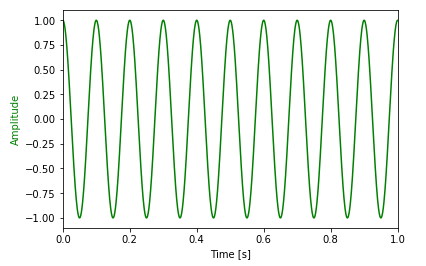
\includegraphics[scale = 1]{original_signal.png} %this is useful too \includegraphics[width = \linewidth]
	\caption{Original signal, from equation \ref{eqn:signal} \cite{notebook:sampling}.}
	\label{fig:signal_og}
\end{figure}    

This is the true function of the signal, but it may be unknown to those wishing to record it.  Say we sample this signal at 18 Hz.  We get the following alias:

\begin{equation}
x[n]=cos(2\pi\dfrac{10n}{18})
\end{equation}
\begin{equation}
x[n]=cos(10\pi\dfrac{n}{9})
\end{equation}
\begin{equation}
x[n]=cos(10\pi\dfrac{n}{9}-2\pi n)
\end{equation}
\begin{equation}
x[n]=cos(10\pi\dfrac{n}{9}-\dfrac{18\pi n}{9})
\end{equation}
\begin{equation}
x[n]=cos(-8\pi\dfrac{n}{9})
\end{equation}
\begin{equation}
x[n]=cos(8\pi\dfrac{n}{9})
\end{equation}

Since a full period is \(2\pi\), we have aliasing (in our example, we have an aliase of \(8\pi\dfrac{n}{9}\).  Our sample rate of 18Hz is too low. Below is our sampling overlaid on the original curve.

\begin{figure}[H]
	\centering
	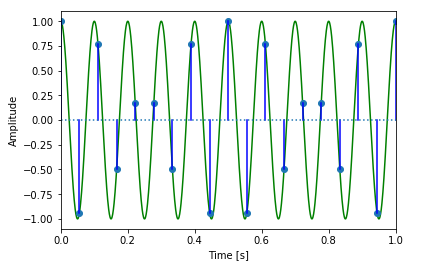
\includegraphics[scale = 1]{sub_sample.png} %this is useful too \includegraphics[width = \linewidth]
	\caption{Overlaid sampling (in blue) on the original curve (in green) \ref{eqn:signal} \cite{notebook:sampling}.}
	\label{fig:sub_sample}
\end{figure}    

As aforementioned, aliasing means that there are additional functions that can cross through the sampling points of our original signal. In the graph below, notice that a new red curve appears, and that it interesects the blue sampling points like our original green signal.

\begin{figure}[H]
	\centering
	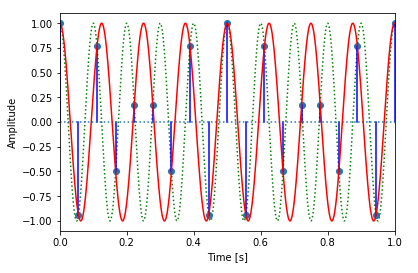
\includegraphics[scale = 1]{aliased_curve.png} %this is useful too \includegraphics[width = \linewidth]
	\caption{The aliased signal (in red) intersects the original signal (in green) at the sampling points (in blue) \ref{eqn:signal} \cite{notebook:sampling}.}
	\label{fig:aliase}
\end{figure}  

So, if our objective is to sample as little as possible, how do we determine the minimum rate necessary?  For perfect reconstruction (of the original signal from the sample), we need:

\begin{equation}
2f_{max}\leq f_{s}.
\label{eqn:nyq}
\end{equation}

This equation says that the frequency rate should be greater than or equal to twice the maximum frequency in the true signal.  But, how do we know the maximum frequency of an unknown signal? We use a function called the sinc function, and take a rectangular pulse of the signal.  The local maxima and minima of the unnormalized sinc function correspond to its intersections with the cosine function \cite{sinc:wiki}.  This means, that we can back-calculate the maximum frequency of an unknown signal through the use of the FFT.  Then, we can calculate the sampling rate of this using formula \ref{eqn:nyq}.

In our case, before processing with a filter, our raw signal had a sampling rate of 44.1 kHz.  This is the standard for CD-quality audio.  We know from Equation \ref{eqn:nyq} that the maximum frequency that can be represented at any given sampling rate is half the sampling rate; thus a 44.1 kHz CD can capture tones up to 22.05 kHz.  This is often over-kill, since as previously mentioned, humans often cannot hear beyond 15 kHz.  We have space to trim that down, but we must make sure to use filters to prevent aliasing.
